\documentclass[10pt,pdf,hyperref={unicode}]{beamer}

\mode<presentation>
{
\usetheme{boxes}
\beamertemplatenavigationsymbolsempty

\setbeamertemplate{footline}[page number]
\setbeamersize{text margin left=0.5em, text margin right=0.5em}
}

\usepackage[utf8]{inputenc}
\usepackage[english, russian]{babel}
\usepackage{bm}
\usepackage{multirow}
\usepackage{ragged2e}
\usepackage{indentfirst}
\usepackage{multicol}
\usepackage{subfig}
\usepackage{amsmath,amssymb}
\usepackage{enumerate}
\usepackage{mathtools}
\usepackage{comment}
\usepackage{multicol}

\usepackage[all]{xy}

\usepackage{tikz}
\usetikzlibrary{positioning,arrows}

\tikzstyle{name} = [parameters]
\definecolor{name}{rgb}{0.5,0.5,0.5}

\usepackage{caption}
\captionsetup{skip=0pt,belowskip=0pt}

\newtheorem{rustheorem}{Теорема}
\newtheorem{russtatement}{Утверждение}
\newtheorem{rusdefinition}{Определение}

% colors
\definecolor{darkgreen}{rgb}{0.0, 0.2, 0.13}
\definecolor{darkcyan}{rgb}{0.0, 0.55, 0.55}

\AtBeginEnvironment{figure}{\setcounter{subfigure}{0}}

\captionsetup[subfloat]{labelformat=empty}

%----------------------------------------------------------------------------------------------------------

\title[Дистилляция]{Стратегии инвестирования с использованием моделей машинного обучения}
\author{К.\,М.\,Баязитов}

\institute[]{Московский физико-технический институт}
\institute[]{Выпускная квалификационная работа\\09.04.01~--- Информатика и вычислительная техника\\Научный руководитель: В.\,А. Ильницкая}
\date[2022]{\small 20\;июня\;2024\,г.}

%---------------------------------------------------------------------------------------------------------
\begin{document}

\begin{frame}
\titlepage
\end{frame}

%----------------------------------------------------------------------------------------------------------
\section{Слайд об исследованиях}
\begin{frame}{Слайд об исследованиях}

\begin{block}{Цель исследования~---}
Повышение качества моделей прогнозирования временных рядов на примере курса акций. 
\end{block}

\begin{block}{Предположение~---}
Внешние факторы, влияющие на курс акций, заложены в ответы опытных инвесторов.
\end{block}

\begin{block}{Решение}
Предлагается при обучении моделей использовать помимо данных временного ряда также агрегированные ответы опытных инвесторов.
\end{block}

\end{frame}

%---------------------------------------------------------------------------------------------------------
\section{Модель автоследования}
\begin{frame}{Модель автоследования}

Автоследование --- способ инвестирования, при котором все желающие могут подключиться к стратегии более опытного инвестора (он же автор стратегии) и автоматически повторять все его сделки на своем счете. 

\[\text{Ответ инвестора} = \frac{\text{Сумма сделки}}{\text{Объем портфеля}}\]

Путем усреднения ответов инвесторов о продаже или покупке акций составляется временной ряд $a_{0}, ..., a_{N}, a_{i} \in [-1, 1]$.

\begin{figure}[h!t]\center
{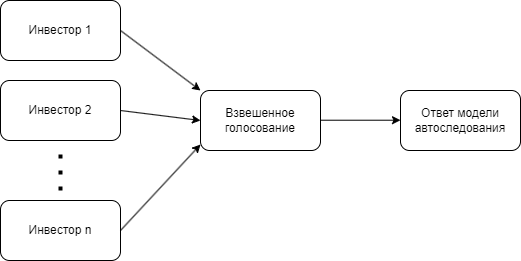
\includegraphics[width=0.6\textwidth]{results/voting.png}}
\end{figure}

\end{frame}

%------------------------------------------------------------------------------------------------------

%---------------------------------------------------------------------------------------------------------
\section{Постановка задачи прогнозирования}
\begin{frame}{Постановка задачи прогнозирования}

$y_{1}, y_{2}, ..., y_{T} $ - временной ряд, $y_{i} \in \mathbb{R}^{n}$.

\bigskip

Требуется получить модель временного ряда:
$$\hat{y}_{t+k}(\mathbf{w}) = f_{t,k}(y_{t-M+1}, ..., y_{t}; \mathbf{w})$$
$$k = 1, ..., K,$$
где  \\
$M$ - размер окна, \\
$K$ - горизонт прогнозирования, \\
$\mathbf{w}$ - вектор параметров модели.

Функция потерь $\mathcal{L}$, используемая при обучении модели:
\[
\begin{aligned}
    \mathcal{L}(\mathbf{w, Y}) =& \sum\limits_{t=M}^{T-K}\sum\limits_{k=1}^{K}(f_{t,k}(y_{t-M+1}, ..., y_{t}; \mathbf{w})-y_{t+k})^{2},
\end{aligned}
\]

Оптимизационная задача:
$$\hat{\mathbf{w}} = \arg\min_{\mathbf{w} \in \mathbb{W}} \mathcal{L}(\mathbf{w, Y}).$$

\end{frame}

%----------------------------------------------------------------------------------------------------------
\section{Экспериментальные данные}
\begin{frame}{Экспериментальные данные}

Эксперимент проводится для данных курса акций YNDX.

Задается временной ряд 
$$x_{0}, x_{1}, x_{2}, ... x_{N}, \quad x_{i} \in \mathbb{R}^{5}$$
$$
    x_{i} = 
    \begin{bmatrix}
        c_{i} & o_{i} & h_{i} & l_{i} & a_{i}
    \end{bmatrix}^{T},
$$
где \\
$c_{i}$ - цена закрытия, \\
$o_{i}$ - цена открытия, \\
$h_{i}$ - максимальная цена, \\
$l_{i}$ - минимальная цена, \\
$a_{i}$ - ответ модели автоследования ($a_{i} = 0$ в базовом варианте обучения модели)

\end{frame}

%----------------------------------------------------------------------------------------------------------
\section{Стационарность}
\begin{frame}{Стационарность}

Ряд приводится к стационарному виду следующими преобразованиями: \\
1) Дифференцирование: $y'_{t} = y_{t} - y_{t-1}$ \\ 
2) Сезонное дифференцирование $y''_{t} = y'_{t} - y'_{t-s}, \ s=5$ \\

\begin{figure}[h!t]\center
\subfloat[]
{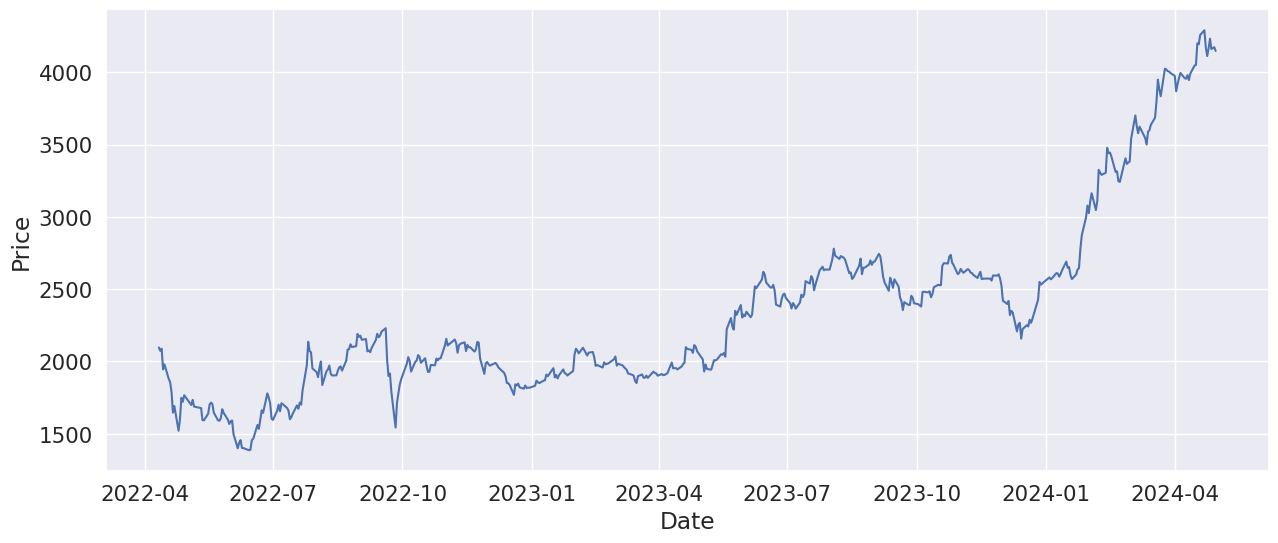
\includegraphics[width=0.5\textwidth]{results/yndx.png}}
\subfloat[]
{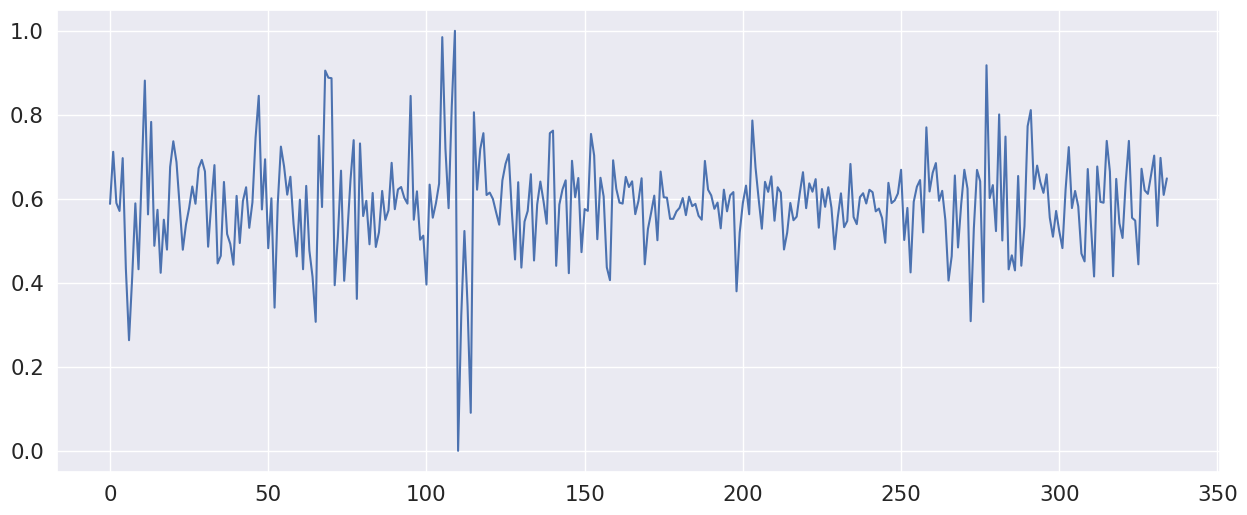
\includegraphics[width=0.5\textwidth]{results/yndx_stationary.png}}
\end{figure}

Для проверки ряда на стационарность используется критерий KPSS: \\
Для исходного ряда $p-value < 0.01$ \\
Для полученного ряда $p-value > 0.01$ 

\end{frame}

%----------------------------------------------------------------------------------------------------------
\section{Составление выборки}
\begin{frame}{Составление выборки}

Методом скользящего окна составляется выборка $\mathfrak{D}=(\mathbf{X},\mathbf{Y})$:

\begin{figure}[h!t]\center
{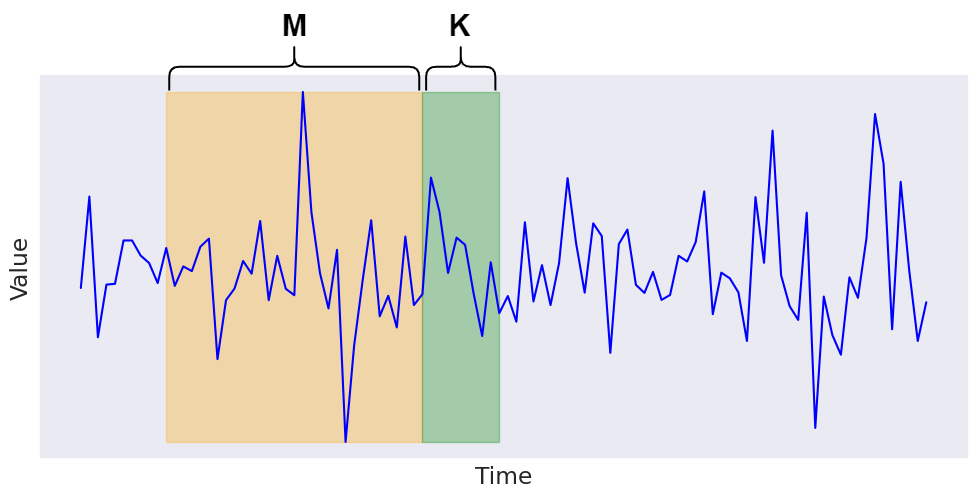
\includegraphics[width=0.45\textwidth]{results/slidingwindow.png}}
\end{figure}

\[
\small
\mathbf{X} = 
\begin{pmatrix}
x_{0} & x_{1} & ... & x_{M}\\
x_{1} & x_{2} & ... & x_{M+1} \\
x_{2} & x_{3} & ... & x_{M+2} \\
\vdots & \vdots & \vdots & \vdots \\
x_{N-K-M} & x_{N-K-M+1} & ... & x_{N-K} \\
\end{pmatrix},
\mathbf{Y} = \begin{pmatrix}
c_{M+1} & c_{M+2} & ... & c_{M+K}\\
c_{M+2} & c_{M+3} & ... & c_{M+K+1} \\
c_{M+3} & c_{M+4} & ... & c_{M+K+2} \\
\vdots & \vdots & \vdots & \vdots \\
c_{N-K+1} & c_{N-K+2} & ... & c_{N} \\
\end{pmatrix},
\normalsize
\]

где  $M$ - размер окна, $K$ - горизонт прогнозирования.

\bigskip

В соотшении 80/20 выборка делится на обучающую и тестовую части.

\end{frame}

%----------------------------------------------------------------------------------------------------------
\section{Выбор размера окна}
\begin{frame}{Выбор размера окна}

В качестве базовой модели используется Seq2Seq архитекутра на основе LSTM.

На графиках показаны метрики корреляции Пирсона и среднеквадратичной ошибки в зависимости от размера входного окна.

\begin{figure}[h!t]\center
\subfloat[]
{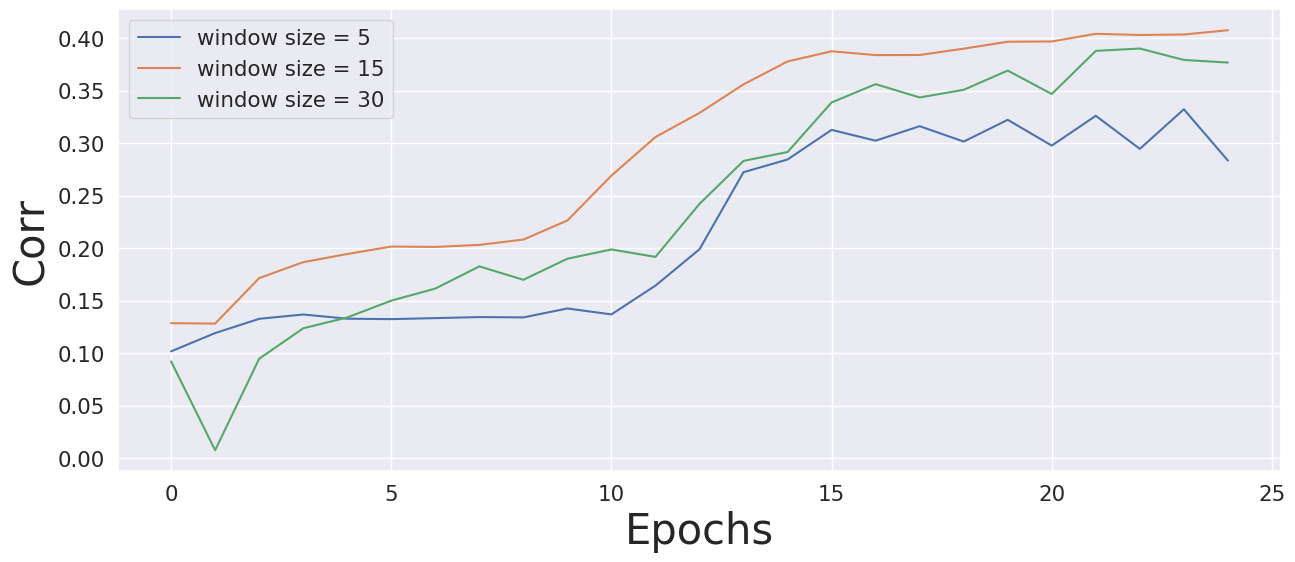
\includegraphics[width=0.45\textwidth]{results/corr_iw.png}}
\subfloat[]
{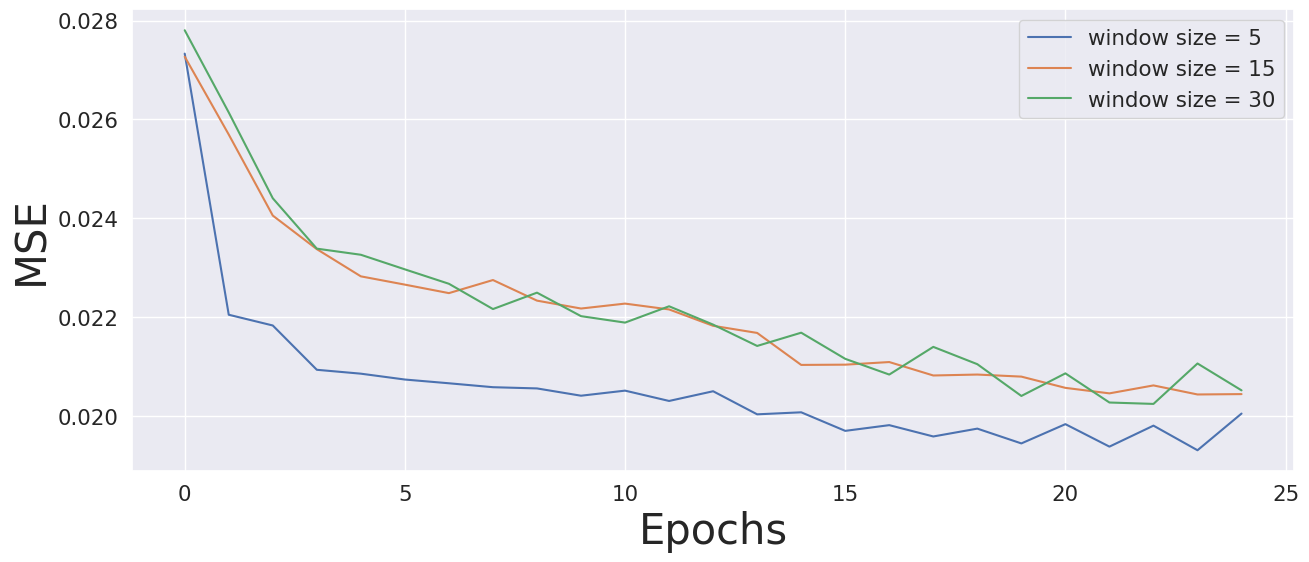
\includegraphics[width=0.45\textwidth]{results/mse_iw.png}}\\
\end{figure}

Визуализация прогнозов моделей:
\begin{figure}[h!t]\center
\subfloat[]
{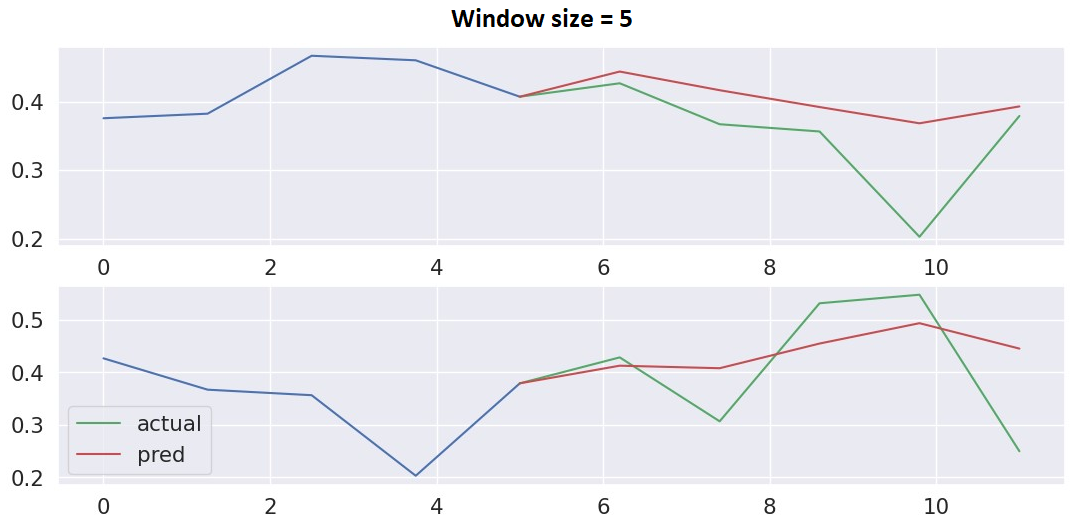
\includegraphics[width=0.4\textwidth]{results/example_iw5.png}}
\subfloat[]
{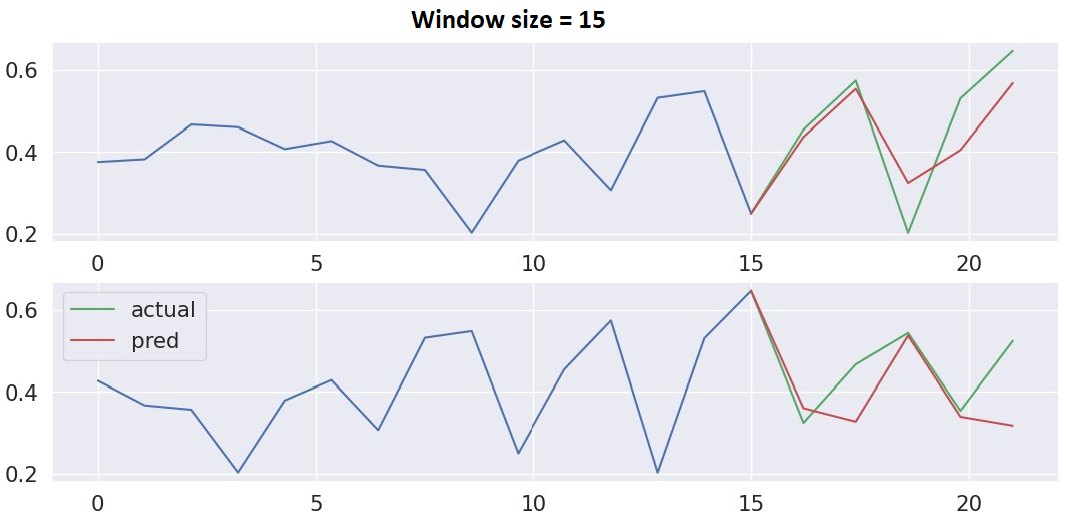
\includegraphics[width=0.4\textwidth]{results/example_iw15.png}}\\
\end{figure}

\end{frame}

%----------------------------------------------------------------------------------------------------------
\section{Выбор горизонта прогнозирования}
\begin{frame}{Выбор горизонта прогнозирования}

На графиках показаны метрики корреляции Пирсона и среднеквадратичной ошибки в зависимости от горизонта прогнозирования.

\begin{figure}[h!t]\center
\subfloat[]
{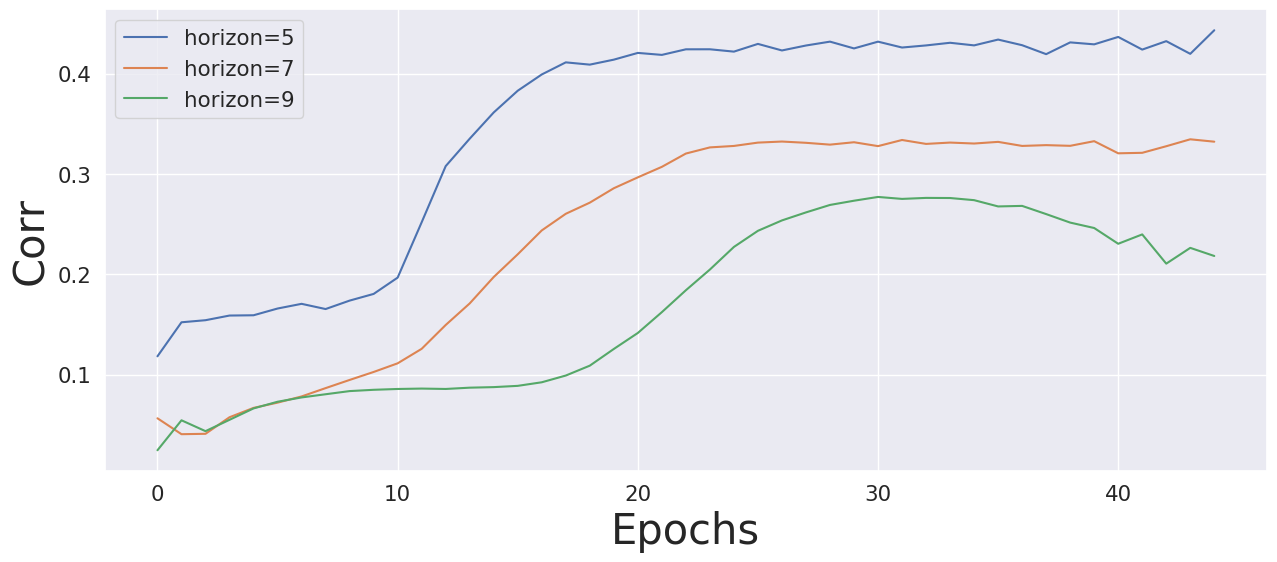
\includegraphics[width=0.45\textwidth]{results/corr_horizon.png}}
\subfloat[]
{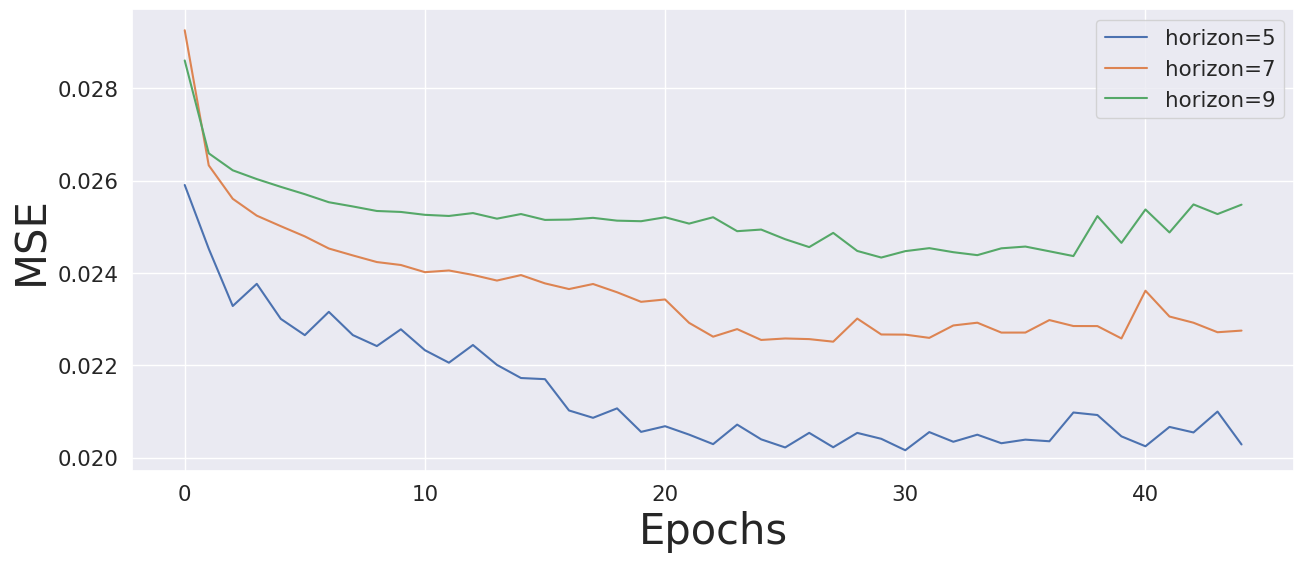
\includegraphics[width=0.45\textwidth]{results/mse_horizon.png}}\\
\end{figure}

С увеличением горизонта прогнозирования качество модели ухудшается.

\end{frame}

%----------------------------------------------------------------------------------------------------------
\section{Анализ предложенного метода}
\begin{frame}{Анализ предложенного метода}

Проводится сравнение базовой модели с моделями, где в качестве дополнительных данных используются:
\begin{enumerate}[1)]
    \item Ответы модели автоследования
    \item Нормальный шум $ \mathcal{N}(0, 1) $
\end{enumerate}

На графиках показаны метрики корреляции Пирсона и среднеквадратичной ошибки.

\begin{figure}[h!t]\center
\subfloat[]
{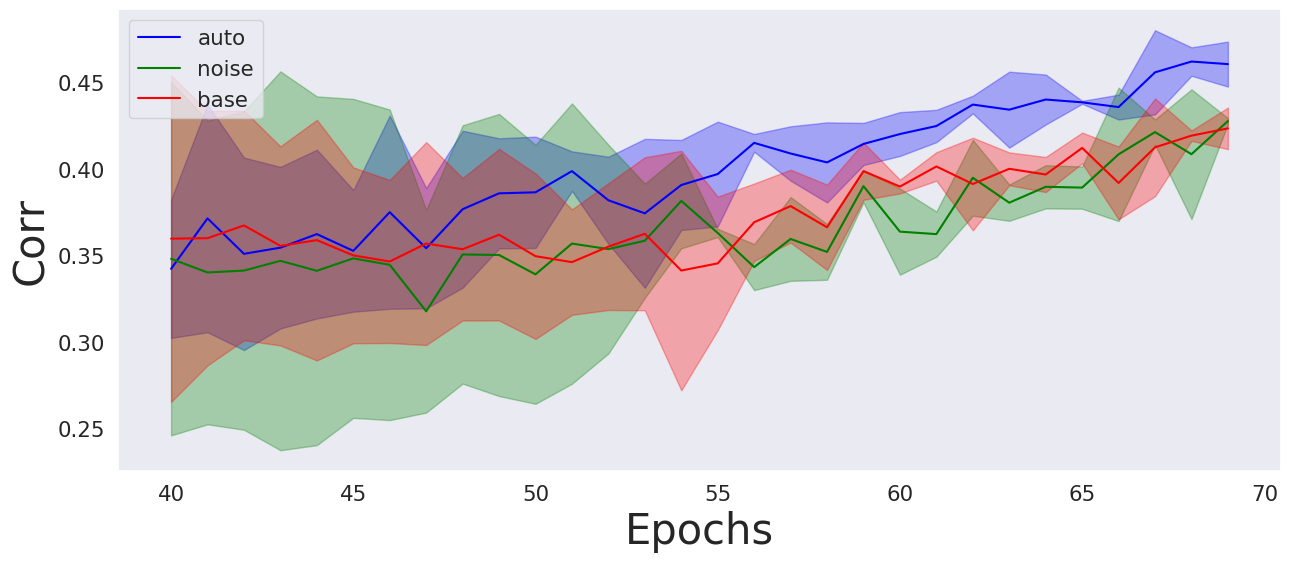
\includegraphics[width=0.45\textwidth]{results/corr.png}}
\subfloat[]
{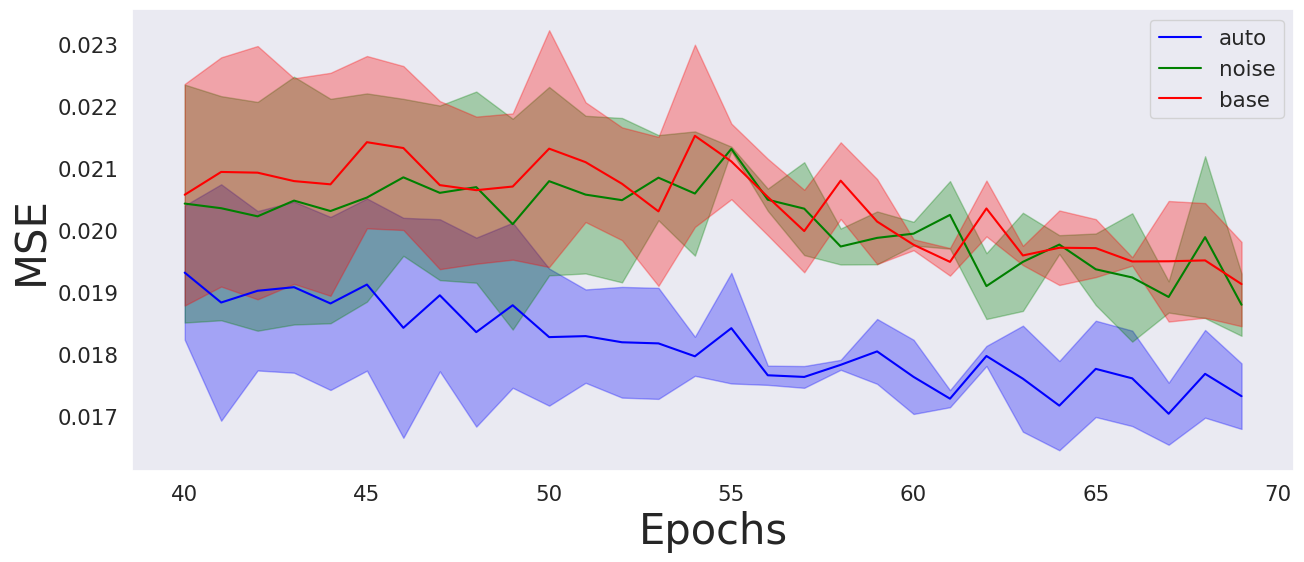
\includegraphics[width=0.45\textwidth]{results/loss.png}}\\
\end{figure}

Модель, использующая ответы модели автоследования, показывает лучшее значение метрик.

\end{frame}

%----------------------------------------------------------------------------------------------------------
\section{ARIMA}
\begin{frame}{ARIMA}

Порядок модели выбирается на основе критерия AIC.

\bigskip

Модель обучается на первых 80 \% данных. Зафиксированные параметры используются для оценки качества прогнозирования на N шагов на оставшихся 20 \% данных.

\end{frame}

%----------------------------------------------------------------------------------------------------------
\section{Сравнение результатов}
\begin{frame}{Сравнение результатов}

\begin{table}[h!t]
\begin{center}
\begin{tabular}{|c|c|c|}
\hline
        \multicolumn{1}{|c|}{Модель} 
        & Корреляция Пирсона & MSE \\
        \hline
        \hline
        Seq2Seq & 0.424 & 0.019 \\
        & (+0 \%) & (-0 \%) \\
        \hline
        Seq2Seq & 0.461 & 0.017 \\
        + Автоследование & (+8.7 \%) & (-10.5 \%) \\
        \hline
        ARIMA & - & - \\
        &  &  \\
\hline
\end{tabular}
\end{center}
\end{table}

\end{frame}

%----------------------------------------------------------------------------------------------------------

%----------------------------------------------------------------------------------------------------------
\section{Выводы}
\begin{frame}{Выводы}

\begin{enumerate}
    \item Предложен метод повышения качества модели при использовании дополнительных данных.
    \item Предложен метод агрегации знаний опытных инвесторов.
    \item Проведен вычислительный эксперимент на реальных данных курса акций YNDX.
    \item Проведен анализ выбора размера окна и горизонта прогнозирования.
\end{enumerate}
 
\end{frame}

%----------------------------------------------------------------------------------------------------------

\end{document}